%%
%% This is file `sample-sigconf.tex',
%% generated with the docstrip utility.
%%
%% The original source files were:
%%
%% samples.dtx  (with options: `sigconf')
%% 
%% IMPORTANT NOTICE:
%% For the copyright see the source file.
%% 
%% Any modified versions of this file must be renamed
%% with new filenames distinct from sample-sigconf.tex.
%% 
%% For distribution of the original source see the terms
%% for copying and modification in the file samples.dtx.
%% 
%% This generated file may be distributed as long as the
%% original source files, as listed above, are part of the
%% same distribution. (The sources need not necessarily be
%% in the same archive or directory.)
%%
%% The first command in your LaTeX source must be the \documentclass command.
\documentclass[sigconf]{acmart}

%%
%% \BibTeX command to typeset BibTeX logo in the docs
\AtBeginDocument{%
  \providecommand\BibTeX{{%
    \normalfont B\kern-0.5em{\scshape i\kern-0.25em b}\kern-0.8em\TeX}}}

%% Rights management information.  This information is sent to you
%% when you complete the rights form.  These commands have SAMPLE
%% values in them; it is your responsibility as an author to replace
%% the commands and values with those provided to you when you
%% complete the rights form.
% \setcopyright{acmcopyright}
% \copyrightyear{2020}
% \acmYear{2020}
% \acmDOI{10.1145/1122445.1122456}

%% These commands are for a PROCEEDINGS abstract or paper.
\acmConference[Explainability '20]{Explainability '20: ACM Symposium on Neural Model Explanations}{December 16--20, 2020}{Karlsruhe, DE}
\acmBooktitle{Explainability '20: ACM Symposium on Neural Model Explanations,
December 16--20, 2020, Karlsruhe, DE}
% \acmPrice{15.00}
% \acmISBN{978-1-4503-XXXX-X/18/06}

% imports
\usepackage{todonotes}
\usepackage{amsmath}

% macros etc
\newcommand{\norm}[1]{\left\lVert#1\right\rVert}
\newcommand{\subsectitle}[1]{\noindent\textbf{#1}}
\DeclareMathOperator*{\argmax}{arg\,max}

\begin{document}

%%
%% The "title" command has an optional parameter,
%% allowing the author to define a "short title" to be used in page headers.
% \title{Manipulating Model Explanations: How to fool what tries to make sense of}
\title{Manipulating Model Explanations: Why you shouldn't trust me}
% A survey on adversarial model interpreter manipulations

\author{Verena Heusser}
\email{verena.heusser@student.kit.edu}
\affiliation{%
  \institution{Karlsruhe Institute of Technology (KIT)}
  \city{Karlsruhe}
  \country{Germany}
}


\begin{abstract}
  This paper reviews state-of-the-art approaches to model explanations with a focus on those techniques that try to 
  fool these methods. 

  We don't only want the model to be good. We want it to be safe and interpretable. 
  As machine learning models enter critical areas in human lives such as the criminal justice system, medicine or financial systems, the inability for humans to understand these models is dangerous and problematic. Advances in the rising research area of explainable AI seems to be a remedy. However, there is not yet a consensus about the validity and robustness of explanations methods themselves. The main suggestion of this paper is to be cautious about results of explanation methods. Explanations can be fooled just as the underlying machine learning models. So. in the end the question must be posed whether inexplainable mdoels should be used at all if we need other models to explain these models but are not valid themselves .. % TODO loop structire aufbauen

\end{abstract}

%%
%% The code below is generated by the tool at http://dl.acm.org/ccs.cfm.
%% Please copy and paste the code
%%
\begin{CCSXML}
  % <ccs2012>
  % <concept>
  % <concept_id>10010147.10010257.10010293.10010294</concept_id>
  % <concept_desc>Computing methodologies~Neural networks</concept_desc>
  % <concept_significance>500</concept_significance>
  % </concept>
  % </ccs2012>
\end{CCSXML}

% \ccsdesc[500]{Computer systems organization~Embedded systems}
% \ccsdesc[300]{Computer systems organization~Redundancy}
% \ccsdesc{Computer systems organization~Robotics}
% \ccsdesc[100]{Networks~Network reliability}

%%
%% Keywords. The author(s) should pick words that accurately describe
%% the work being presented. Separate the keywords with commas.
\keywords{Interpretability, Neural networks, adversarial training}

%% A "teaser" image appears between the author and affiliation
%% information and the body of the document, and typically spans the
%% page.

\maketitle


% manipulating explanations and explaining manipulations
\section{Introduction}
\label{sec:introduction}
% questioning the how

In recent years deep learning models have demonstrated superior performance in a number of tasks. While the performance is still rising and more task domains are accomplished, these models still remain black boxes often uninterpretable even by experts. 
In many domains, neural networks currently are the state-of-the-art solution. However, their superior performance comes at the cost of complexity, as the models often employ millions to even billions of parameters in order to achieve universal function approximation. This complexity means a drawback in interpretability as the decision making process of such a network cannot be followed by humans without the help of further tools. For instance, withing object recognition one would like to assume that the presence (or absence) of an object in the image causes a model to decide for a specific object category, closely akin to how humans base their decision process. 

At present, many concerns regard the coherence of automated decisions to ethical standards. Regarding the expanding number of tasks that automated computer algorithms are used for nowadays, this concern is becoming even more important, as machine learning models are moving out of the lab into the real world. The application of algorithms for prediction of recidivism rates are already applied at court \cite{chouldechova2017fair}, and the filtering of job applicants, piloting of self-driving cars, diagnoses of diseases or automated food recognition \cite{ruede2020multi} are already in use.

% sort of prove that neural networks make a safe decision without biases

% much broader context to create security and large scale applications 

% https://dl.acm.org/doi/pdf/10.1145/3387514.3405859?casa_token=lCc16GOTZsEAAAAA:gypLNU1o2Wwl3wt_b8stRbb0mgxEomX8PWprPeciNdkhVften3-5E01RM50e0W9NGQaGd4TrLOhA

% explainability can be viewed as an active characteristic of a model, denoting any action orprocedure taken by a model with the intent of clarifying or detailing its internal functions.


Thus, automated interpretation methods are required to make sense of the reasoning process and stability of such deep learning based models and to ensure that a model makes decisions without unfair or hidden biases. 
The research field approaching the explanation or validation of machine learning models is called explainable artificial intelligence (XAI).
%  not knowing why models decide
Not knowing about the biases of a network the vastly advancing technology of machine learning to be used in high-stakes and safety critical applications and prevent real-life deployment of such systems. 
Furthermore, the rise in machine learning model deployments also caused the development of adversarial attacks. These attacks attempt to fool a machine learning model by providing deceptive input. Fooling refers to the resulting malfunction of the model. 
% TODO first example

Not knowing about attacks and data arranged to exploit specific vulnerabilities has contributed to a relatively new research field of XAI comprising topics of (1) \textit{model explanations}, (2) \textit{adversarial attacks}, or manipulation methods and (3) the field of \textit{adversarial manipulations of model explanations}. All of this is also known by the name of robust machine learning or even explainable artificial intelligence, as all subfields have the common goal to make models more robust and safe for deployment. 
(1) refers to the development of techniques that can be used to understand and explain the decision making process of a machine learning model or even the development of models that are inherently interpretable. (2) is the field of detecting vulnerabilites in models that cause models to be deceived by altered input. 
(3) is the main topic of this paper, i.e. how to fool explanation models in order to detect vulnerabilities and malfunctions in explanation methods. 

Detecting such vulnerabilities in models is most crucial 

Fragility limits how much wecan trust and learn from the interpretations



% While most of the approaches to explainability focus on the application to computer vision tasks, other domains are seldomly chosen. 
Most research on explainability focuses on the application of computer vision tasks. 
% todo cite a lot here
% https://www.bmc.com/blogs/machine-learning-interpretability-vs-explainability/ 
Most works in the field of XAI focus on image classification task, mostly because visualizations of a neural networks prediction can be easily verified by a human. The general purpose of image classification is to detect what objects are in an image. If a model works can be checked rather easily (if an image contains a cat, the prediction of a neural network should be cat and not some other object category). However, how it works (\textit{interpretability}), i.e. based on which features in the image the decision is made or which parameters in the model influence the prediction most, is an entirely different matter (\textit{explainability}).  


More importantly, while a big motivation for the development of robust and explainable systems is to overcome biases in models, datasets with 
direct implication of biases are seldomly used and by far not treated as benchmarking scenarios for explainability analyses.  


% Theoretical background
% why do adv attacks make sense? most models are trained on iid samples and thus not directly applicable to the real world, as the real world violates this statistical assumption. 




% Outline
The overview presented in this article examines the existing literature and contributions in the field of XAI focusing on methods to manipulate explanation methods.  
The critical literature analysis might serve as a motivation and step towards the biggest problems in XAI: How to make sure that interpretations of models are truly valid. 
This paper is structured as follows... 


\section{Interpretation Methods}
\label{sec:interpretation_methods}

There exists a variety of definitions in the vastly expanding research field of XAI, and the concept of \textit{interpretability} still has no formal commonly used technical meaning \cite{lipton2018mythos}. To build on the common ground of existing research, this work follows the terminology of Lipton et al. \cite{lipton2018mythos} and Arrieta et al. \cite{arrieta2020explainable}.

Broadly, interpretabiity focuses on \textit{how} and \textit{why} a machine learning model makes predictions.
Simply put, interpretability is focused on getting some notion of an explanation for the decisions made by a machine learning model.

%%%%%%%%%%%%%%%%%%%%%%%%%%%%%%%%%%%%%%%%%%%%%%
\subsection{Terminology}
\label{subsec:interpretation_methods_terminology}
The authors of \cite{arrieta2020explainable} make a distinction between the related but different concepts of \textit{interpretability} and \textit{explainibility}. Lipton \cite{lipton2018mythos} further breaks down interpretability into \textit{transparency} and \textit{post-hoc} interpretability. The notion of \textit{explainibility} from \cite{arrieta2020explainable} can be related to Liptons's \textit{transparency}, while Lipton's \textit{post-hoc} interpretability is essentially \textit{interpretability} as defined by Arrieta et al. \cite{arrieta2020explainable}.

\mypar{Post-hoc Interpretability} refers to the the extent to which cause and effect can be observed in a model, which can be translated to uncovering \textit{why} a model made prediction $y$ to an input $\mathbf{x}$, or how input and output ralate. Consider the example of image classification from \autoref{fig:bb}. Here, interpretability would mean that if a cat is present in the image (the cause), the model classifies it to the category 'cat' (the effect). Now imagine we find that the model takes the green meadow in the image as evidence to predict 'cat', and not the cat itself. This would imply a lack of interpretability, as the model learns to assign features to the concept 'cat' other than those related to 'cat' in the correct sense. This toy example emphasizes a common problem in image classification: \cite{xiao2020noise} observe the over-reliance of models on image background, rather than on objects in the foreground. % Note that interpretabe AI cannot verify if the learned relationships between features and outputs is truly causal (tha meadow in tha image can be correlated to the image category, e.g. when most images depictiong a cat shows cats on green meadows. This is a correlation of features but not necessarily a causilaty in tha sense of 'meadow --> cat'. ) https://www.pnas.org/content/pnas/116/44/22071.full.pdf causal inference
% Simply put, interpretability is focused on getting some notion of an explanation for the decisions made by a machine learning model.

\mypar{Explainibility or Transparency} on the other hand spans methods to uncover \textit{how} a model makes predictions, meaning to observe the inner workings of a model and thus to literally explain what is happening in terms of understanding of the mechanisms by which a model works. Thus, tansparency refers to the model's inherent properties that can be known before the training process and that are helpful to understand the model.

\par\smallskip
While both concepts seem to be important for the general objective of explainable artificial intelligence, this paper focuses on post-hoc interpretability.
There are essentially two ways to achieve interpretability: (1) to use inherently interpretable models or (2) to post-process a model in a fashion that allows to yield insights. The former is known as the development of \textit{surrogate} models and more generally described as \textit{model-agnostic} methods. Option (2) is known as \textit{model-transparent} methods. 

\mypar{Local and Global Methods.} A further categorization can be made based on the scope of interpretations: \textit{Local} methods aim at providing interpretations that are true for a single data points and its neighbors. 
\textit{Global} methods aim at gaining interpretations that are valid for most data points in a class \cite{kim2018interpretability, nguyen2017plug, yosinski2015understanding}. The interpretation methods discussed within this paper mostly fall into the class of local explanation methods \cite{ribeiro2016should, lundberg2017unified, bach2015pixel}. % TODO add all?

\mypar{Feature Attribution Methods and Sample Attribution Methods. } Interpretation methods aim at making complex and inherently uninterpretable black box models interpretable by creating human readable visualizations. 
A frequently used type of explanation methods are \textit{feature attributions} mapping each input feature to a numeric score. This score should quantify the importance of the feature relative to the model output. The resulting attribution map is then visualized as a heatmap projected onto the input sample. This allows humans to interpret which input attributes are the most helpful for making tha final prediction. Sample attribution methods on the other hand interpret the model performance in terms of the importance of training examples from the dataset. 

We propose the following formal definition for interpretation method:\newline

\textbf{Definition 1: Interpretation Method.}

\setlength{\leftskip}{0.39cm}

  \noindent We consider a neural network $N: \mathbb{R}^d \to \mathbb{R}^k$. For the an arbitrary classification task, $N$ classifies an input sample $\mathbf{x}\in \mathbb{R}$ in $k$ categories where the prediction $f_N(\mathbf{x})=y \in \{1, ..., K\}$ is given by $y = arg max_i f_N(\mathbf{x})_i$.

  Given the neural network $N$, it's input vector $\mathbf{x} \in \mathbb{R}^d$ and the the neural networks prediction for input $\mathbf{x}$, $f_N(\mathbf{x})=y$, an interpretation method $\mathcal{I}$ determines why label $y$ has been chosen by $N$ for input $\mathbf{x}$. 
  The interpretation is given by an output vector $\mathbf{h_k} \in \mathbb{R}^d$ for a class $k$ where each entry $h_i$ is mostly a numeric value describing the relevance for the $i$-th input feature $x_i$ of $\mathbf{x}$ for the final score $f_N(\mathbf{x})$.

\setlength{\leftskip}{0pt}
\par\smallskip\vspace{-0.1cm}

As $\mathbf{h}$ has the same dimensions as the input $\mathbf{x}$ it can be mapped to the input, overlaying $\mathbf{x}$ as a heatmap, where the color value represents the importance of feature $x_i$ towards the prediction $f_N(\mathbf{x})$.
An example is given in \autoref{fig:lrp_cat_lrp}. Higher values, implying a stronger relative importance for making the prediction $f_N(\mathbf{x})$, are depicted in dark red. 

% A model-transparent interpretation method, in the following named interpreter $\mathcal{I}$, generates a heatmap
%  $$h_c^\mathcal{I}(\boldsymbol{\omega}) = \mathcal{I}(\mathbf{x}, c; \boldsymbol{\omega})$$
%   for a neural network with parameters $\boldsymbol{\omega}$ and class $c$. The heatmap is a vector $h_c^\mathcal{I}(\boldsymbol{\omega}) \in \mathbb{R}^d$, where the $j$-th value $h_{c, j}^\mathcal{I}(\boldsymbol{\omega})$ represents the importance score of the $j-th$ input feature $x_j$ for the final score of class $c$.

While all explanation methods try to obtain importance measures for the network prediction, they differ with respect to how these measures are obtained. \cite{evaluating_explanations_security} propose two major categories for interpretation strategies, namely \textit{black-box}, in the following named \textit{model-agnostic} methods and \textit{white-box}, or \textit{} interpretation methods. 
While black-box interpretations assume no knowledge about the underlying model, white-box methods only work by using the model parameters. 

This terminology of discriminating between black-box and white-box methods may not be confused with the nature of the underlying models: Models still remain of black-box nature even though a white-box method may contribute to making the decision making process of such a model more insightful. % The opposite ofblack-box-nessistransparency,i.e., the search for a direct understanding of the mechanism by which a model works [5] 


The following section details the two categories and will give examples of the state-of-the-art interpretation methods within each group. 

% \noindent\textbf{Black-box Methods.} Black-box interpretations assume no knowledge about the model thus treating it as a black-box. The underlying model is approximated by learning it's behavior with an interpretable model, e.g. a linear model. As the model itself does not need to be known for using such a model-agnostic approach, thy can be used in scenarios where the model itself is not directly accessible. A black-box interpretation offers the big advantage to be applicable to any model.


% \noindent\textbf{White-box Methods.} On the other side are white-box interpretations, where the model is known with all its parameters. Thus, the explanations can be directly computed by using the model instead of relying on an approximation of $f_N$ as within the black-box models. As within these white-box models, tha model parameters can be used for calculating the interpretations, these methods are also named gradient or saliency map based methods. 

\subsection{Model-agnostic methods.}
\label{subsec:bb_methods}

% https://proceedings.neurips.cc//paper/2020/file/2c29d89cc56cdb191c60db2f0bae796b-Paper.pdf p. 4 
Model-agnostic interpretations assume no knowledge about the model thus treating it as a black box. The underlying model is approximated by learning it's behavior with an interpretable model, e.g. a linear model. The interpretable model is also dubbed the 'surrogate' model. The common approach for learning the surrogate is to approximate the relationship between the input samples and the corresponding prediction by tho model.
As the model itself does not need to be known, these approaches can be used in scenarios where the model itself is not directly accessible. Model-agnostic interpretations are fairly popular and are used in a wide range of applications, ranging from finance and law to medicine and chemistry \cite{elshawi2019interpretability, whitmore2016mapping}. 

A black-box interpretation offers the great advantage of being applicable to any model and offers simplicity because the interpretation is embedded in the model. However, this option of gaining interpretability might be costly for users that already have a high performing model. For this reason, growing need for methods exists that can be applied without retraining or modifying the underlying model.
We will briefly describe two common model-agnostic approaches. Refer to the original papers for details.

\mypar{Local Interpretable Model-agnostic Explanations (LIME).}\newline
LIME \cite{ribeiro2016should} perturbs the input and observes how the predictions of a black box model change. For the task of image classification, LIME creates a set of perturbed instances by dividing the input image into interpretable components, which are technically contiguous superpixels, and runs each perturbed instance through the model to get the probability for how much the change in each superpixel influences the whole model prediction. 

\autoref{fig:lime_cat} shows an example of LIME applied to the neural network model Inception-v3 \cite{szegedy2016rethinking}. Input image from the ImageNet dataset \cite{ILSVRC15}. The superpixel in dog instances place is highlighted in green, which correctly indicates that this superpixel has a high influence on the prediction of the images correct class ('bernese mountain dog'). LIME also correctly indicates that the superpixel in the cat's place does not indicate the correct class label.

\begin{figure}[ht]
  \centering
  \begin{subfigure}{0.32\linewidth}
    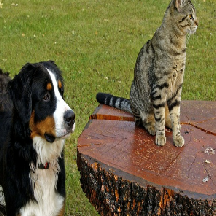
\includegraphics[width=\linewidth]{figures/lime_orig.png}
    \caption{Original}
    \label{fig:bird-a}
  \end{subfigure}
  \begin{subfigure}{0.32\linewidth}
    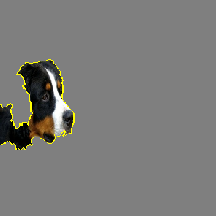
\includegraphics[width=\linewidth]{figures/lime_dog_mask.png}
    \caption{Mask.}
    \label{fig:bird-a}
  \end{subfigure}
  \begin{subfigure}{0.32\linewidth}
    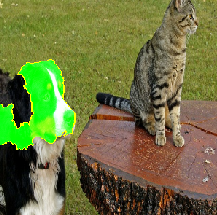
\includegraphics[width=\linewidth]{figures/lime_dog_map1.png}
    \caption{Saliency Map.}
    \label{fig:bird-a}
  \end{subfigure}
  \caption{Visualization of the output of the LIME interpreter applied to an image and image classification model.}\label{fig:lime_cat}
  \vspace{-0.3cm}
\end{figure}

% https://github.com/marcotcr/lime
% While the model may be very complex globally, it is easier to approximate it around the vicinity of a particular instance. While treating the model as a black box, we perturb the instance we want to explain and learn a sparse linear model around it, as an explanation. The figure below illustrates the intuition for this procedure. The model's decision function is represented by the blue/pink background, and is clearly nonlinear. The bright red cross is the instance being explained (let's call it X). We sample instances around X, and weight them according to their proximity to X (weight here is indicated by size). We then learn a linear model (dashed line) that approximates the model well in the vicinity of X, but not necessarily globally.


\mypar{SHapley Additive exPlanations (SHAP).} SHAP \cite{lundberg2017unified} builds on Shapley analysis, which is essentially about judging the importence of attibutes. The model is trained on a number of subsets of all available features, and the feature importance scores are calculated by evaluating the effects that the omissions of the specific features have on the model prediction. An example is shown in \autoref{fig:shap_dog}. Image regions highlighted in green are found to be important for predicting the correct label.

\begin{figure}[ht]
  \centering
  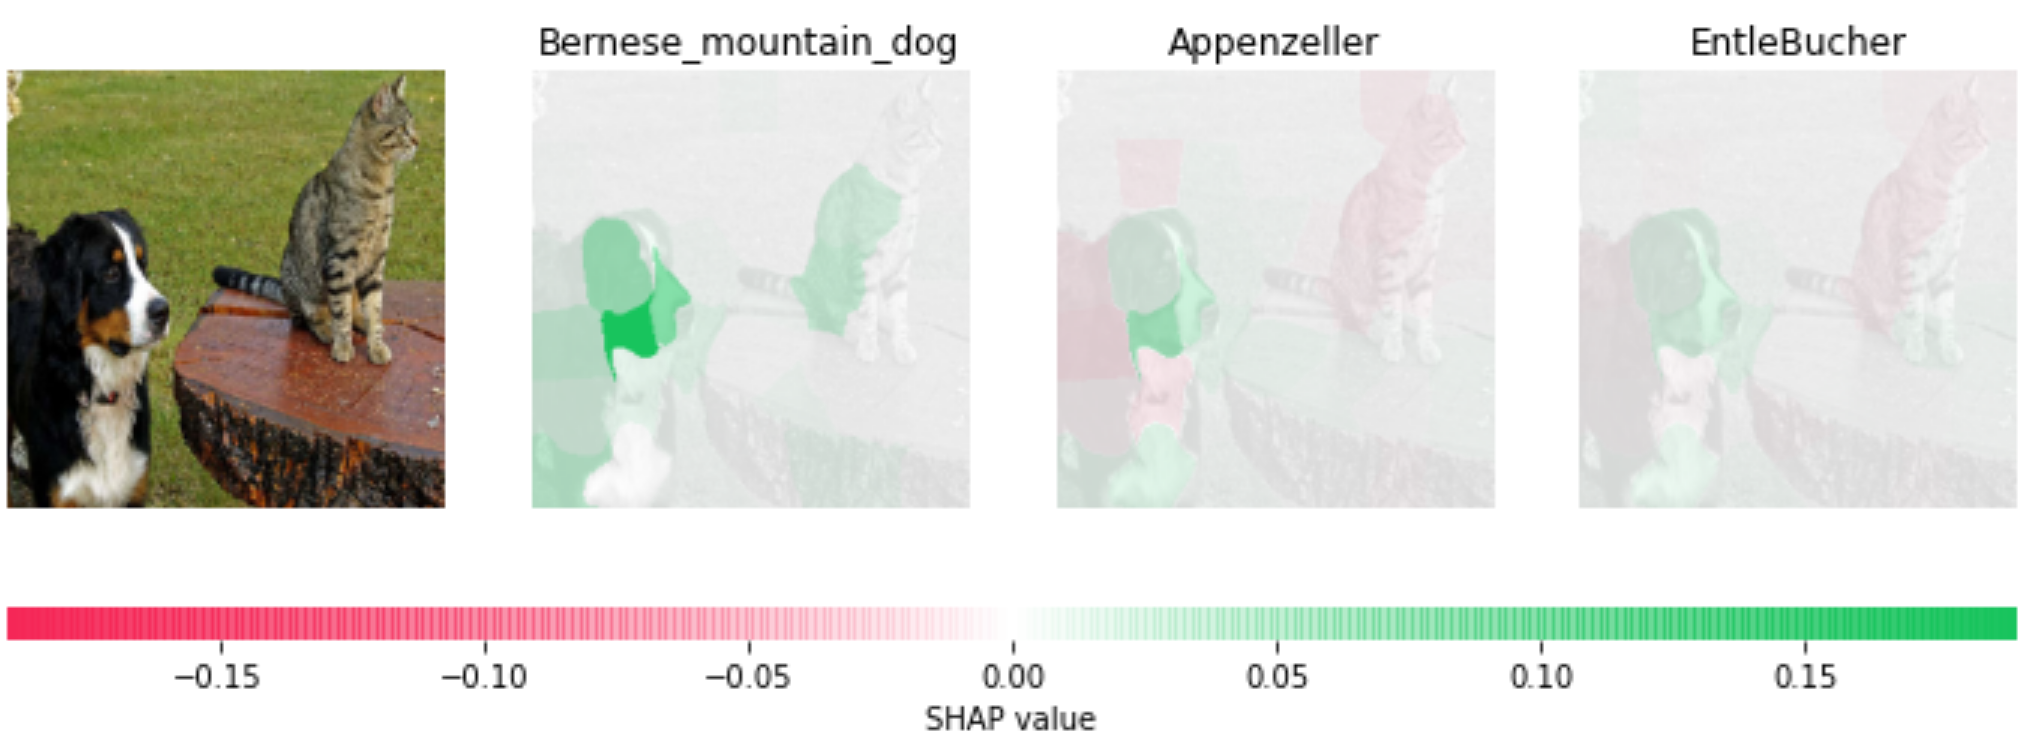
\includegraphics[width=\linewidth]{figures/cat_dog_shap.png}
  \caption{Visualization of the output of the SHAP interpreter applied to applied to an image and image classification model.}\label{fig:shap_dog}
  \vspace{-0.3cm}
\end{figure}


\subsection{Model-transparent methods.}
\label{subsec:wb_methods}

The other group of interpretations are model-transparent, or white-box methods, where the underlying model is known with all its parameters. Thus, the interpretation can be directly computed by using the model instead of relying on an approximation of $f_N$ as within the black-box methods. These methods typically rely on the relationship between an input sample, the underlying model's prediction and the associated activations of the models hidden layers. Methods within this group are for example propagation-based and gradient-based approaches. The former propagate back the model's prediction back through the model. The latter make use of the information provided by the gradients of the loss function, which contain sensitive information about the prediction and the features. Using the backpropagation method, features in the input can be highlighted based on the amount of gradient they receive. This shows their contribution to the final score. 
A few example methods within this group are listed below. 

\mypar{Layer-wise Relevance Propagation (LRP).} While many approaches in the group of model-transparent interpretations are designed only for image classification, or convolutional neural networks, this method \cite{bach2015pixel} is an exception. LRP propagates relevance values backwards through the network and decomposes the score of a predicted class backwards through the network. It relies on a Taylor series close to the prediction point rather than partial derivatives at the prediction point itself. An example for a feature map produced by LRP can be found in \autoref{fig:lrp_cat_lrp}.
%The output is a heatmap of relevance values, depicting for each feature how helpful or harmful the feature is for predicting the target class. 

\mypar{DeepLIFT} \cite{shrikumar2017learning} is an improved version of LRP, where a reference point in the input feature space is defined. Relevance scores are propagated proportionally to the changes of neuronal activations from the reference. % https://arxiv.org/pdf/1710.10547.pdf

\mypar{SmoothGrad (SG)} \cite{smilkov2017smoothgrad} avarages over interpretations of noisy copies of an input sample thus reducing noise by visually diffusing the interpretation. The noise is drawn from i.i.d. from a normal distribution. 

Methods developed for convolutional neural networks are for instace GradCAM \cite{selvaraju2017grad} or SimleGrad TODOcite. 
% \mypar{Gradient-weighted Class Activation Mapping (Grad-CAM)}
% Grad-CAM \cite{selvaraju2017grad} uses the gradients of any target concept, flowing into the final convolutional layer to produce a coarse localization map, highlighting the important regions in the image for predicting the concept.

% \mypar{SimpleGrad (SimpleG)}

% Please see the original publications for more detailed information. 

\section{Manipulation Methods}
\label{sec:manipulation_methods}

As outlined in \autoref{sec:interpretation_methods}, there are a variety of explanation methods readily available as frameworks and open source implementations. However, there is still little analysis on the robustness and reliability of such methods. 
While it is already common practice to test machine learning models against adversarial attacks in a number of domains \cite{gao2019universal, kereliuk2015deep}, the same is not yet the standard for interpretation methods. We argue that interpretation techniques should not be used in critical applications without basic testing of interpretation techniques against adversarial settings.

\subsection{Adversarial Setting}
\label{subsec:adversarial_setting}
\mypar{Adversarial Attacks on Models. }
Adversarial examples, as first introduced by \cite{szegedy_intriguing}, are clever manipulations of an input by an adversary which aims at causing misclassification and fooling of applications. They are mostly used to fool or attack machine learning models. We formally define adversarial attacks by the following properties: 
\par\smallskip
\textbf{Definition 2: Model Manipulation Method}
\begin{enumerate}
    \item[1.] \textit{Impercpetibility of Perturbation}: The adversal example is similar to original data, i.e. the norm of the added perturbation $\delta$ to an input sample $\mathbf{x}$ thus must be small, i.e. $$\norm{\mathbf{x}+\delta} = \norm{(\mathbf{x}+\delta)-\mathbf{x}}_{\inf} \leq \epsilon$$
    \item[2.] \textit{Prediction dissimilarity}: The prediction of the model is significantly different to the prediction on the non-adversarial example: $$f_N(\mathbf{x}+\delta) \approx f_N(\mathbf{x})$$
\end{enumerate}
Note, that within adversarial foolings of models, the perturbation is mostly applied to the input data, and not to the model itself.

% TODO cite
Evidence from many studios shows that deep learning models can be easily tricked by adversarial examples. 
Albeit there are not yet as many studies, there also exists evidence that many interpretation methods are also fragile with respect to small changes to input data \cite{adebayo2018sanity, samek2019explainable, alvarez2018towards} as well as to the model itself \cite{fooling_nn_interpreters,dimanov2020you}. This fooling of interpretation methods is outlined below. 

\mypar{Adversarial Attacks on Model Interpreters. } 
Contrary to adversarial attacks on machine learning models, the focus of this paper is on the attacks on interpretation techniques without changing the prediction of the model. 
An adversarial attack on a model interpretation is in the following also called a \textit{manipulation} method. 
The goal is to apply perturbations to either an input sample or the model to change the output of an interpretation technique while leaving the model prediction unchanged. The last condition is important because adversarial interpreter manipulations aim to fool the interpretation method and essentially not the model itself. 
Fooling the model would only disclose the vulnerability of the model but would not allow to gain insight into the stability of the interpretation method. 
Again, the problem can be formally defined as:

% A manipulation method refers to a method influencing an interpretation method $\mathcal{I}$ to yield a wrong interpretation. This influence on the interpretation method is also called \textit{fooling} or an \textit{attack}. 
\par\smallskip
\textbf{Definition 3: Interpretation Manipulation Method.}

\setlength{\leftskip}{0.39cm}
% as it is the goal to disclose the vulnerability of the explanation method and not the vulnerability of the model.
\noindent A manipulation method $\mathcal{F}$ is defined as a method for altering the output of an explanation method $\mathcal{I}$ while leaving the model performance of the neural network $N$ roughly unchanged. 
As manipulations can be applied on the input or the model level (see \autoref{subsec:manipulation_levels}), $\mathbf{x}+\delta$ denotes a perturbed input sample regarding the input level manipulation, while $N+\delta$ denotes a model with altered parameters, referring to the model level manipulation.

A manipulation method is successful in fooling an interpreter, if the following properties hold: 
\begin{enumerate}
    % TODO for all i, as in http://lcfi.ac.uk/media/uploads/files/DimanovBhattJamnikWeller_YouShouldntTrustMe.pdf 
    \item[1.] \textit{Prediction similarity}: The model prediction stays approximately the same, i.e. $$f_N(\mathbf{x}+\delta) \approx f_N(\mathbf{x}) \text{, or } f_{N+\delta}(\mathbf{x}) \approx f_N(\mathbf{x})$$
    \item[2.] \textit{Interpretation dissimilarity}: The explanation map $h(\mathbf{x}+\delta)$ is significantly different to the explanation map resulting from non adversarial models or inputs $h(\mathbf{x})$, i.e. $h(\mathbf{x}+\delta)$ or $$\argmax_{\delta} = \mathcal{D}(\mathcal{I}(x_i, \boldsymbol{\omega}), \mathcal{I}(x_i+\delta, \boldsymbol{\omega})$$
    \item[3.] \textit{Impercpetibility of Perturbation}: In case the attack is in the input domain of the model, the perturbation of input samples must be imperceptible by humans. According to \cite{dombrowski2019explanations}, the norm of the added perturbation $\delta$ to an input sample $\mathbf{x}$ thus must be small, i.e. $$\norm{\mathbf{x}+\delta} = \norm{(\mathbf{x}+\delta)-\mathbf{x}}_{\inf} \leq \epsilon$$ % https://arxiv.org/pdf/1710.10547.pdf 
\end{enumerate}
\setlength{\leftskip}{0cm}

These measures are to be seen as comparison between a baseline model $N$ and a model that is applied an the adversarial setting (i.e. either $N$ is not changed but applied to adversarially altered data $x+\delta$, or $N$ is adversarially trained thus becoming $N+\delta$). 

\cite{dimanov2020you} extend these properties to include the so called \textit{model similarity}. This measure extends the \textit{prediction accuracy} to span the accuracy difference in between the baseline model and the new model, and also the mismatch of data points where the predictions of both models differ. 


%%%%%%%%%%%%%%%%%%%%%%%%%
\subsection{Taxonomy of Interpretation Manipulation Methods}
\label{subsec:taxonomy_manipulations}
There are two important categories of Manipulation Methods that aim at attacking model interpretation methods. The first category is based on the level these manipulations operate on, i.e. input space level or model / paramater level. 
The second categorization is based on the target of the manipulations. While untargeted manipulations are mostly random perturbations, targeted manipulations aim to perturb the interpretation of specific input features. 

%%%%%%%%%%
\subsubsection{Manipulation Levels}
\label{subsubsec:manipulation_levels}
\par\smallskip
\noindent 

\par\smallskip
\noindent\textbf{Adversarial Input Manipulation.} The general approach is to perturb or alter input data while observing the effect of this perturbation on the model prediction. This concept is visualized in \autoref{fig:input_manipulation}. 
As found in \cite{advlime_aies20}, visually-imperceptible perturbations of an input image can make explanations worse for the same model and interpreter. 

\begin{figure}[ht]
    \centering
    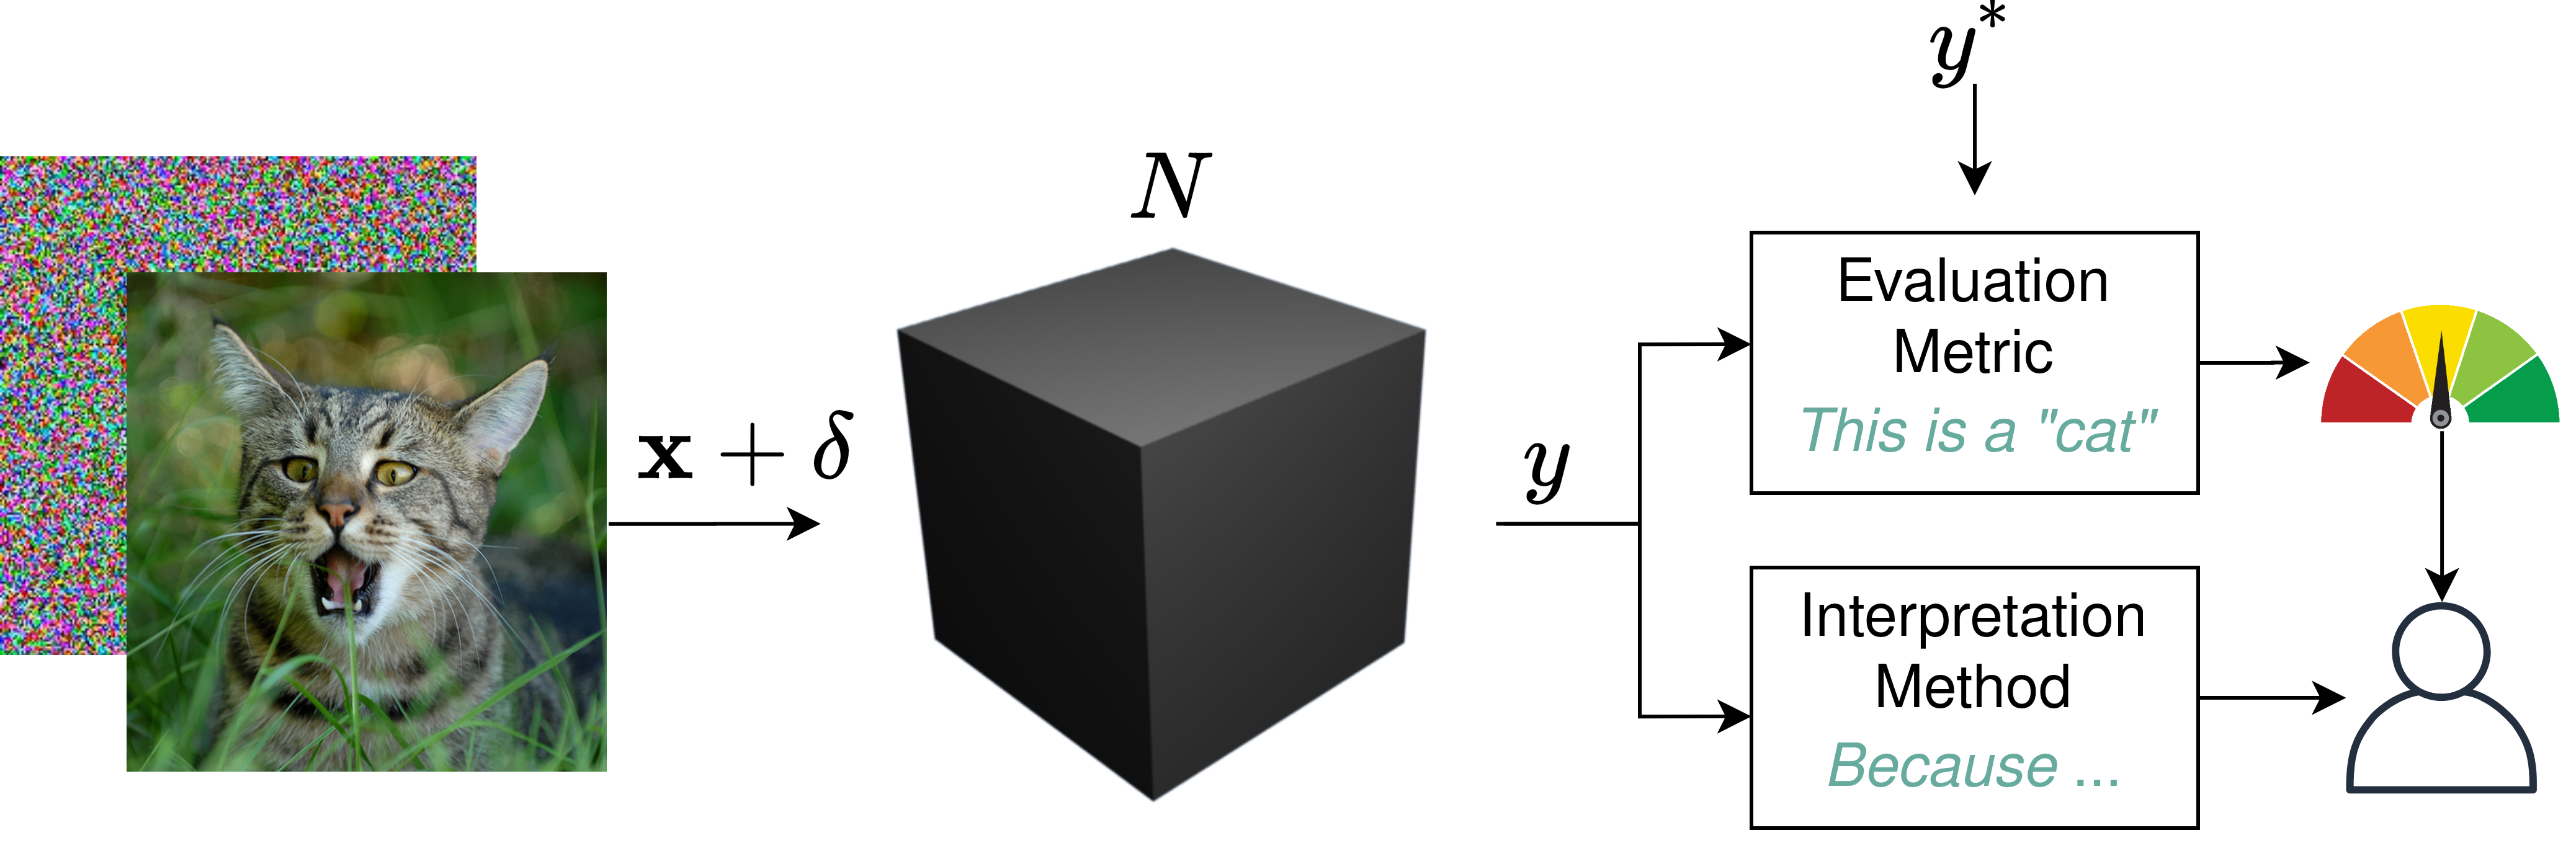
\includegraphics[width=\linewidth]{figures/input_manipulations.png}
    \caption{Depiction of an adversarial input manipulation. The model is fine-tuned with altered input samples, which are indicated by $\mathbf{x}+\delta$.}
    \label{fig:input_manipulation}
    \vspace{-0.3cm}
\end{figure}

\par\smallskip
\noindent\textbf{Adversarial Model Manipulation.} 
Contrary to input manipulations, model manipulations do not operate on the input space but rather on the model parameter space itself. 
As first introduced by Heo et al. \cite{fooling_nn_interpreters} in 2019, this line of research is comparably new. 
Adversarial model manipulations are obtained by fine-tuning the model on the same data but with an adapted objective function. \cite{fooling_nn_interpreters} propose the adapted loss function for the task of image classification of $$ \mathcal{L} = \mathcal{L}_{CE}(\mathcal{D};\omega) + \lambda \cdot \mathcal{L}(\mathcal{D};\omega; \omega_0) $$ where $\mathcal{L}_{CE}$ would be the standard cross-entropy classification loss. 
Adversarial model manipulation is depicted in \autoref{fig:input_manipulation} where the altered model is indicated by $N+\delta$.

\begin{figure}[ht]
    \centering
    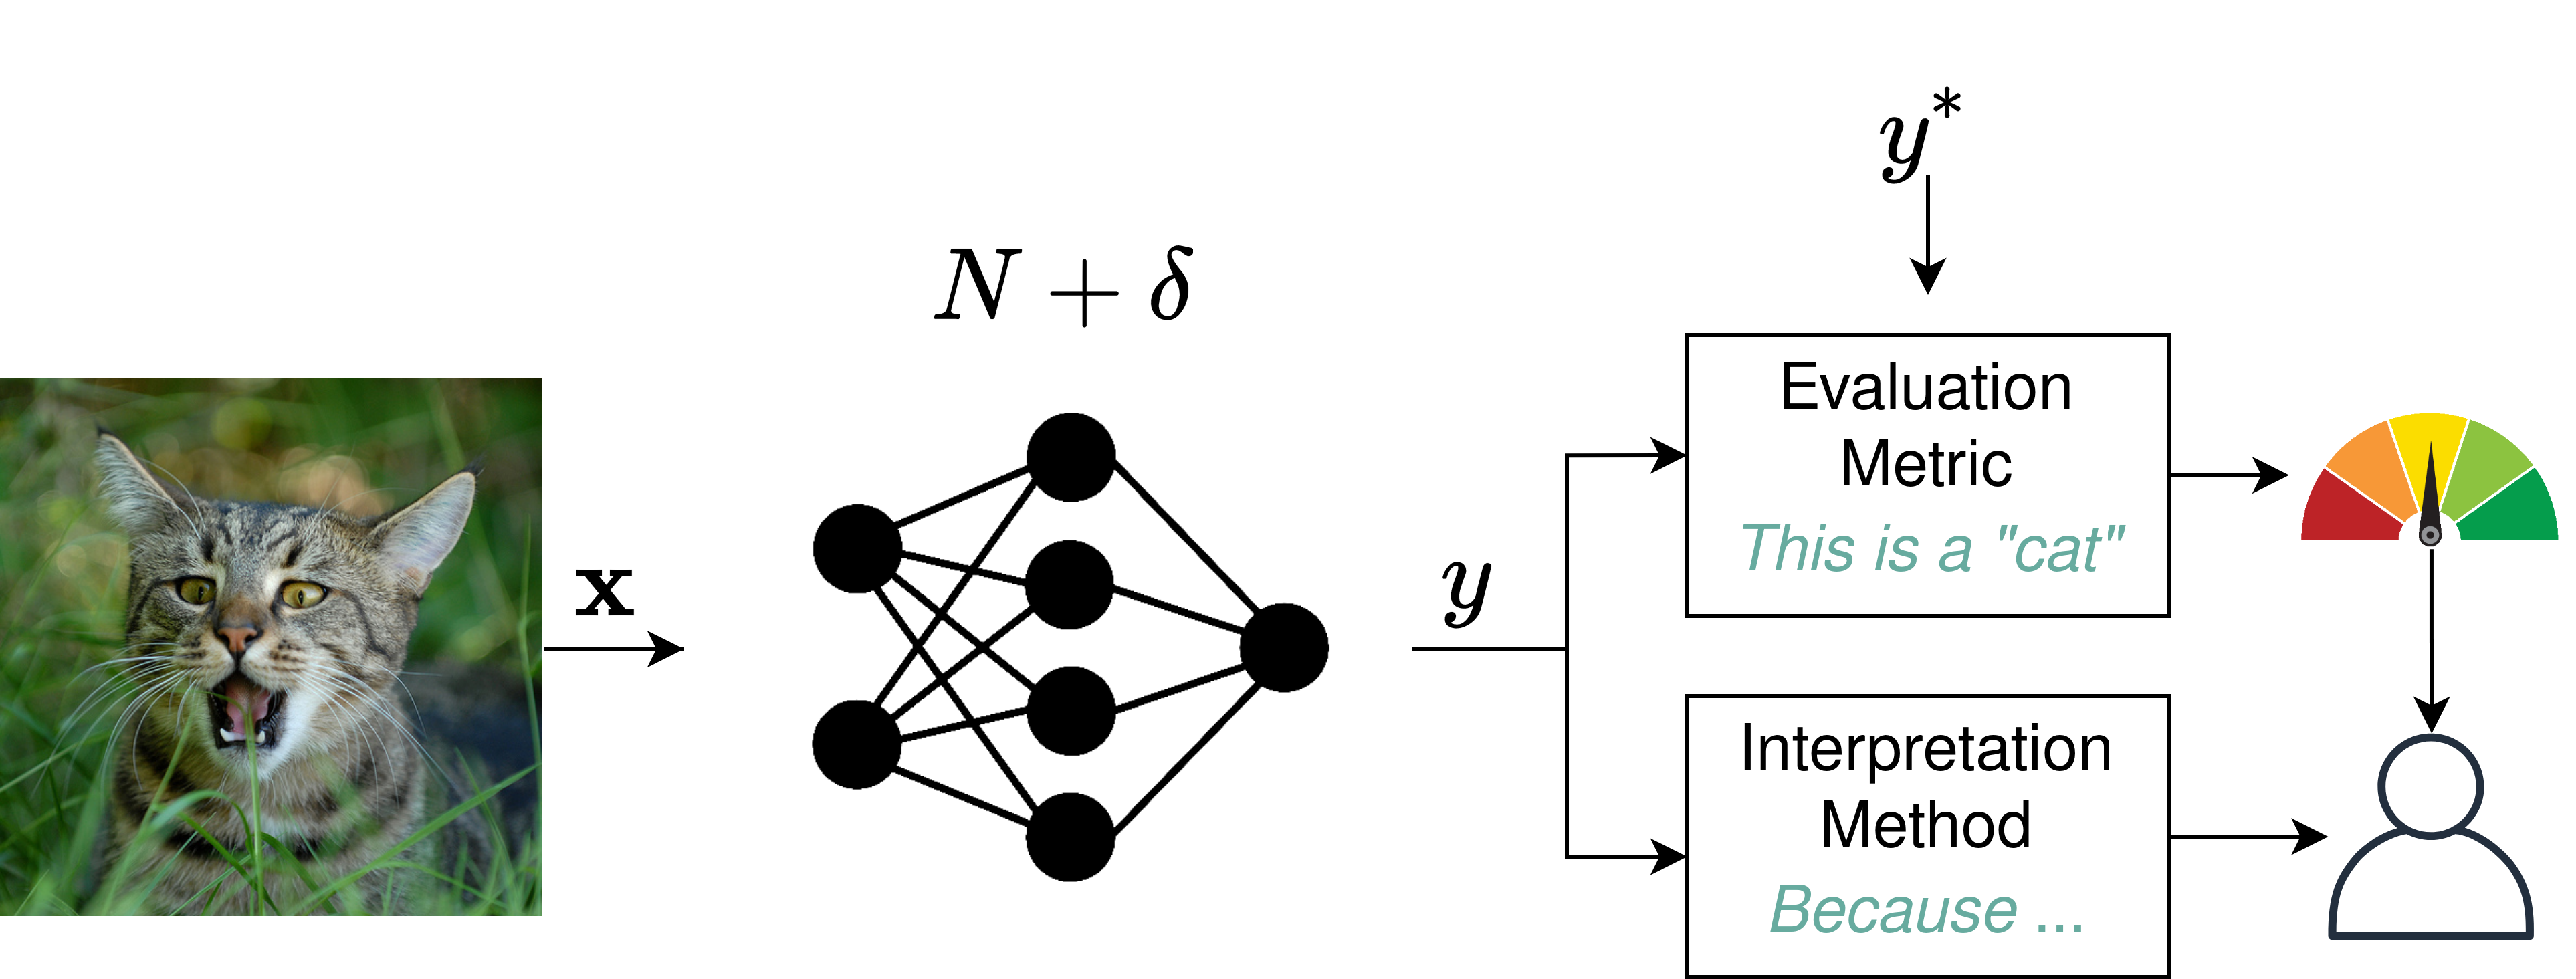
\includegraphics[width=\linewidth]{figures/model_manipulations.png}
    \caption{Depiction of an adversarial model manipulation. The model is fine-tuned with the same distribution of input data and a fooling loss, thus yielding the biased model $N+\delta$.}
    \label{fig:input_manipulation}
    \vspace{-0.3cm}
\end{figure}

%%%%%%%%%%
\subsubsection{Manipulation Targets}
\label{subsubsec:manipulation_targets}

\par\smallskip
\noindent
In addition to the categorization of manipulation methods based on the manipulation level, the methods can further be categorized based on the target of their perturbation. The first possibility is \textit{untargeted} perturbation, the second is \textit{targeted} perturbation. Both these styles can be applied on either model and input level. 

\mypar{Untargeted Manipulations.} 
The majority of manipulations is untargeted, meaning that the applied perturbations are mostly random and not designed to change the prediction for a specific portion of an input sample. 

\mypar{Targeted Manipulations.} 
On the contrary, targeted manipulations are designed to specificly alter the explanation of distinct features of an input instance. Such a specific feature might be an object in the input image in the context of image classification. 
For instance \cite{fooling_nn_interpreters} introduce a fooling scheme in which the interpretations of the target classes elephant and school bus are swapped. 
Manipulations on the level of the model are mostly targeted, as the explanation methods are being fooled by adapting the model parameters. 

% Model manipulations pose a much higher threat for deploying the models: If a model itself is changed to explicitly, systemactically fool an explanation method, the bias of the model is internal and much harder to reveal than just a different sort of input into the model. 

%%%%%%%%%%%%%%%%%%%%%%%%% 
\subsection{Evaluation Criteria}
\label{subsec:eval_criteria_manipulations}
Basides the necessary properties of a successful interpretation manipulation method, other evaluation criteria are importent to access the successfulness of a fooling method and to enable the comparison between different fooling methods. These criteria are infermally defined in the following.

\mypar{Effectiveness.} The manipulation scheme is inexpensive to conduct. Input manipulations are by definition inexpensive, as the perturbation can be applied to single input samples. Model manipulations are more expensive as they require tho model parameters to be adapted. However, an adversarial model can be obtained by fine-tuning the model with an adapted objective function. This fine-tuning also has the advantage that the model is adapted to include a systematic bias and can thus be applied to fool explanation methods without further adapting the model or input samples after the fine-tuning step. Furthermore, this systematic bias is hidden in the model, and is hard to uncover. Input manipulations can only fool the model when the inputs are always manipulated. 

\mypar{Transferability.} The manipulation does not only fool one type of interpretation method, but it's effect transfers to other interpretation techniques. 
% This property is naturally given for the class of model manipulations


\mypar{Generalisation.} Generalization of an attack refers to the transfer of fooling to other test samples. This is noteworthy since a manipulation method might only perturb the decision boundary locally around the training points, i.e. only influencing trainang instances and their neighbors. However, it is desired that the explanations of unseen samples are affected as well. Furthermore, not only unseen samples intarpretations, but also samples that are far away in the feature space, should be affected,
% On the contrary, model manipulations are non-local perturbations, meaning that they do not merely perturb an input sample
% but rather effect all samples in the way that the model itself is changed. 
% TODO iid ood?
% The  generalisation  of  the  attack  to  testpoints  is  noteworthy  since  we  might  expect  that  the  deci-sion boundary would be perturbed locally around the train-ing points to affect only their explanations, without signifi-cant change for test points, especially if far away in featurespace (see Appendix for more)

TODO \\
Most of the explanation methods outlined in sec. \autoref{sec:interpretation_methods} have been shown to be vulnerable to adversarial perturbations. 
Manipulation methods often show that there exist small feature changes resulting in a change of the explanation methods output while the output of the model itself does not change. 
Most approaches aim at providing a relevance measure of the input features. \\



Creation of a fooled model by fine-tuning the model with a fooling loss. 
% https://github.com/rmrisforbidden/Fooling_Neural_Network-Interpretations/blob/master/Materials/PPT.pdf 


As outlined in section \autoref{sec:manipulation_methods}, there exists a plethora of interpretations methods differing in the assumption about the model character and also with respect to how interpretations are obtained. Thus, reliable evaluation methods are required allowing for a choice of an appropriate and robust interpretation method. Ultimately, the accordance to these evaluations should naturally allow for chosing an appropriate and robust intarpretation method.  
Evaluations of the quality of an explanation method are separated into qualitative and quantitative evaluations. 
% \cite{fooling_nn_interpreters} propose to measure the quality of an explanation method by their stability with respect to adversarial model manipulations. 

\mypar{Qualitative Evaluation.} 
Inspection and ramdom sampling are commonly used techniques to obtain an intuition about the effect of manipulations. 
As interpretations are attributed to input features, the resulting relevance values $l$ can be easily mapped to the input vector $\mathbf{x}$. Visual inspection of these evaluations for specific samples is informative, but does not allow for general statistics and validation of manipulation effects. Thus, quantitative evaluations are required. 

\mypar{Quantitative Evaluation.} 
As the goal of interpreter manipulations is to fool an interpreter, thus altering the output of in interpreter, it is straightforward to compare interpretations and data samples before and after perturbation \cite{ghorbani2019interpretation}.
Common metrics for quantitatively measuring similarities are the following: 
\begin{itemize}
    \item \textbf{Spearman's rank order correlation.} As interpretation methods rank the features based on their importance, the rank correlation \cite{spearman1961proof} is a natural meusure for comparing interpretations. 
    \item \textbf{Intersection of the top-$k$ features.} For some tasks, only the top-$k$ features are relevant, such that a comparison between these top-$k$ features is insightful. 
    \item \textbf{Fooling Success Rate (FSR).} \cite{fooling_nn_interpreters} introduce the concept of the Fooling Success Rate (FSR) with the aim to create a measure for systematically measuring the robustness of an interpretation method to adversarial model manipulations. The FSR measures on how many samples from a dataset an interpretation method $\mathcal{I}$ is fooled by a model manipulation. The higher the FSR, the more often an inetpretation method is fooled. 
    \item \textbf{Structural Similarity Index (SSIM).} SSIM values are relative similarity measure in the range $\left[0, 1\right]$, where larger values indicate higher similarity.
    \item \textbf{Pearson Correlation Coefficien (PCC).} PCC is also a relative similarity measure returning values in the range $\left[0, 1\right]$. Larger values indicate higher similarity.
    \item \textbf{Mean Squared Error (MSE).} As an absolute error measure, values close to zero indicate high similarity. 
    \item \textbf{AOPC} TODO
\end{itemize}
\noindent Note that these are only examples without demand for completeness. For further information see \cite{adebayo2018sanity}.
Normalizing these measures to yield values in $\left[0, 1\right]$ with a sum of one is good practice. 


% TODO add methods to reverse / disclose manipulations

\section{Characterization of Robustness}
\label(sec:robustness)

This section introduces common evaluation strategies designed to test the 
robustness of either model or interpreter towards an applied attack. 

TODO: 
- auch auf entlarvungsmethoden eingehen? 



\section{Transferability of Perturbations}
\label(sec:transferability)

input perturbations do not propagate to the whole validation set. 
On the contrary, model manipulations are non-local perturbations, meaning that they do not merely perturb an input sample
but rather effect all samples in the way that the model itself is changed. 


\section{Explaining Manipulations}
\label{sec:explaining_manipulations}

% papers: geometry is to blame

There is an abundance of examples and scenarios where model explanations fail. However, there are few paper specifically targeting why these manipulations work in the first place. 


\section{Sanity Checks for Interpreters}
\label{sec:sanity_checks_for_interpreters}

Checking the robustness, scope and hence the quality of model interpreters has become an indispensable step in explainable machine learning. 

\cite{adebayo2018sanity} propose a number of randomization tests for saliency-map based interpreters.
The authors find that most methods fail their tests, and warn of the danger of visual assessment. 
 



Additionally, in order to account for adversarial model manipulations, Heo et al. \cite{fooling_nn_interpreters} propose to expand the criteria for checking the robustness of interpreters further.

\section{Benchmarking Interpretations}
\label{sec:benchmarking}

Checking the robustness, scope and hence the quality of model interpreters has become an indispensable step in explainable machine learning. 
Evaluating explanation and interpretation methods is difficult as ground truth is mostly lacking. In most applications, it is not known which input features are most important. 

% https://github.com/google-research-datasets/bam 
% https://arxiv.org/abs/1907.09701

\cite{adebayo2018sanity} propose a framework for sanity checking saliency map based interpretation methods. Fer this, a number of randomization tests are introduced along with some visualization techniques and metrics to compare interpretation outputs. The authors find that most methods fail their tests, and warn of the danger of visual assessment. Specifically, they warn that humans tend to chose visually significant appearing images that lack sensitivity to the data distribution and generation as well as to the model. 
However, their findings are so far limited to the domain of computer vision models and tasks. % TODO @outlook
Implementing their randomization tests for other real-world datasets, such as COMPAS \cite{compas_dataset} or the adult income dataset \cite{adult_income} would be an interesting next step. 

Additionally, in order to account for adversarial model manipulations, Heo et al. \cite{fooling_nn_interpreters} propose to expand the criteria for checking the robustness of interpreters further.


\section{Experiments}
\label{sec:experiments}
In this section, several experiments are evaluated that were conducted to replicate findings of other studies. Furthermore these approaches are extended to other domains and datasets. 


\subsection{Explanation Methods}

\subsection{Manipulation Methods}

\subsection{Models}

\subsection{Datasets}

\subsubsection{ImageNet}
\subsubsection{Recidivism Dataset}
\subsubsection{German dataset of..}

\section{Conclusion}
Finally, it must be noted that the suitability of a method depends on its application domain. 


Much critique has been applied to methods aiming at interpreting complex and potentially non-interpretable models. 
Some researchers argue it is not worthwhile to study non interpretable systems while dismissing that using inherently interpretable models in the first place might be the better approach. 

Adversarial attacks show that machine learning systems are still fundamentally fragile: They may be successful in a number of tasks, but fail to adapt to ood scenarios, i.e. when being applied to unfamiliar territory. 
% Our results raise concerns on how interpretations of neural networks can be manipulated.
% fail unpredictably

 The findings about manipulating interpretations do not suggest that interpretations are completely meaningless, just as adversarial attacks on predictions models do not imply that machine learning models are useless. However, they suggest that there still are fundamental flaws in the way neural networks operate und that much caution and supervision sould be applied if they are to be deployed in the real world. 



% \balance
\bibliography{mybib}{}
% \bibliographystyle{plain}
\bibliographystyle{ACM-Reference-Format}


% \appendix

\end{document}
\endinput